\documentclass[11pt]{article}
% Discuss:
% * writing sample
% ** Expanding longer proposal
% ** Work out semantics
% ** Work out syntax
% * letters of rec

\usepackage{geometry}

\usepackage{silence}
\WarningFilter{biblatex}{Patching footnotes failed}
\usepackage[
style=authoryear,
natbib
]{biblatex}
\addbibresource{bibliography.bib}
\setcounter{biburlnumpenalty}{6000}
\setcounter{biburllcpenalty}{7000}
\setcounter{biburlucpenalty}{8000}

\usepackage{graphicx}
\usepackage{caption} % More complex captioning
\usepackage{subcaption} % subfigure environment and co.
\usepackage{placeins} % \FloatBarrier flushes the float buffer

\usepackage{amsmath}
\usepackage{amssymb}
\usepackage{bbold}

\usepackage{tikz}
\usetikzlibrary{positioning}
\usepackage[linguistics]{forest}
\usetikzlibrary{tikzmark}

\usepackage[normalem]{ulem} % \sout strikethrough text

\usepackage{gb4e}

\newcommand{\ok}{\checkmark}
\DeclareMathOperator{\bbexists}{\exists\mskip-7mu\exists}


\title{\vspace{-2cm}The Humantities Institute Undergraduate Research Fellowships 2026-2027 Proposal}
\author{Benjamin Kyle Olson}
\date{\today}

\begin{document}
\maketitle

\section{Introduction}

This senior thesis is to explain relative clauses out of expletive \textit{there} contexts (TRCs) such as (\ref{ex:trc}).\footnote{Much has been abbreviated here from the formal proposal for reasons of space.} These are known to exhibit determiner selection (\ref{ex:det}): broadly, definites and universals are acceptable; indefinites are unacceptable. This is particularly striking against the well-known (anti)definiteness effect (DE) of expletive \textit{there} contexts (TCs) seen in (\ref{ex:def}).

\begin{exe}
	\ex {The cat that there was in the room jumped out the window.}\label{ex:trc}\footnote{\label{fn:intro}TRCs seem to be almost universally partially marked probably due to presentationality. I have plans to resolve this snag.}
	\ex {\textbf{Determiner Selection:} (\cite{carlsonAmountRelatives1977}, ex. 10a, 10e, 11b)
		\begin{xlist}
			\ex[]  {The people there were at that time only lived a few decades.}
			\ex[]  {Every lion there is eats meat.}
			\ex[*] {A man there was disagreed.}
		\end{xlist}}\label{ex:det}
	\ex {\textbf{Definiteness Effect:} (\cite{milsarkExistentialSentencesEnglish1974}, ch. 1, ex. 12a-b)
		\begin{xlist}
			\ex[]  {There will be a duck roasted on Arbor Day.}
			\ex[*] {There will be the duck roasted on Arbor Day.}
		\end{xlist}}\label{ex:def}
\end{exe}

\begin{figure}[htbp]
	\centering
	\begin{minipage}{.8\textwidth}
		\centering
		\begin{subfigure}{.42\textwidth}
			\begin{center}
				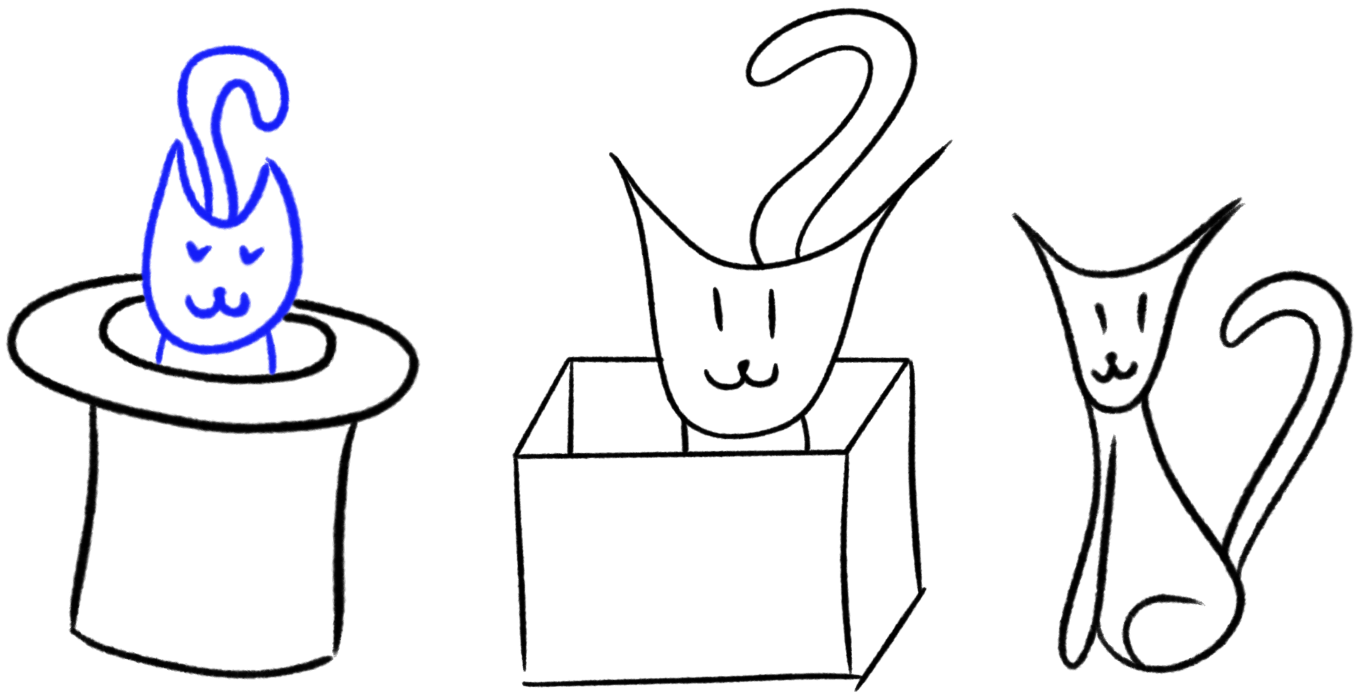
\includegraphics[width=0.95\textwidth]{figures/absolute.png}
				\captionsetup{justification=centering,format=hang}
				\caption{Absolute context, \\ exactly one hat}\label{fig:absolute}
			\end{center}
		\end{subfigure}\ %
		%
		\begin{subfigure}{.57\textwidth}
			\begin{center}
				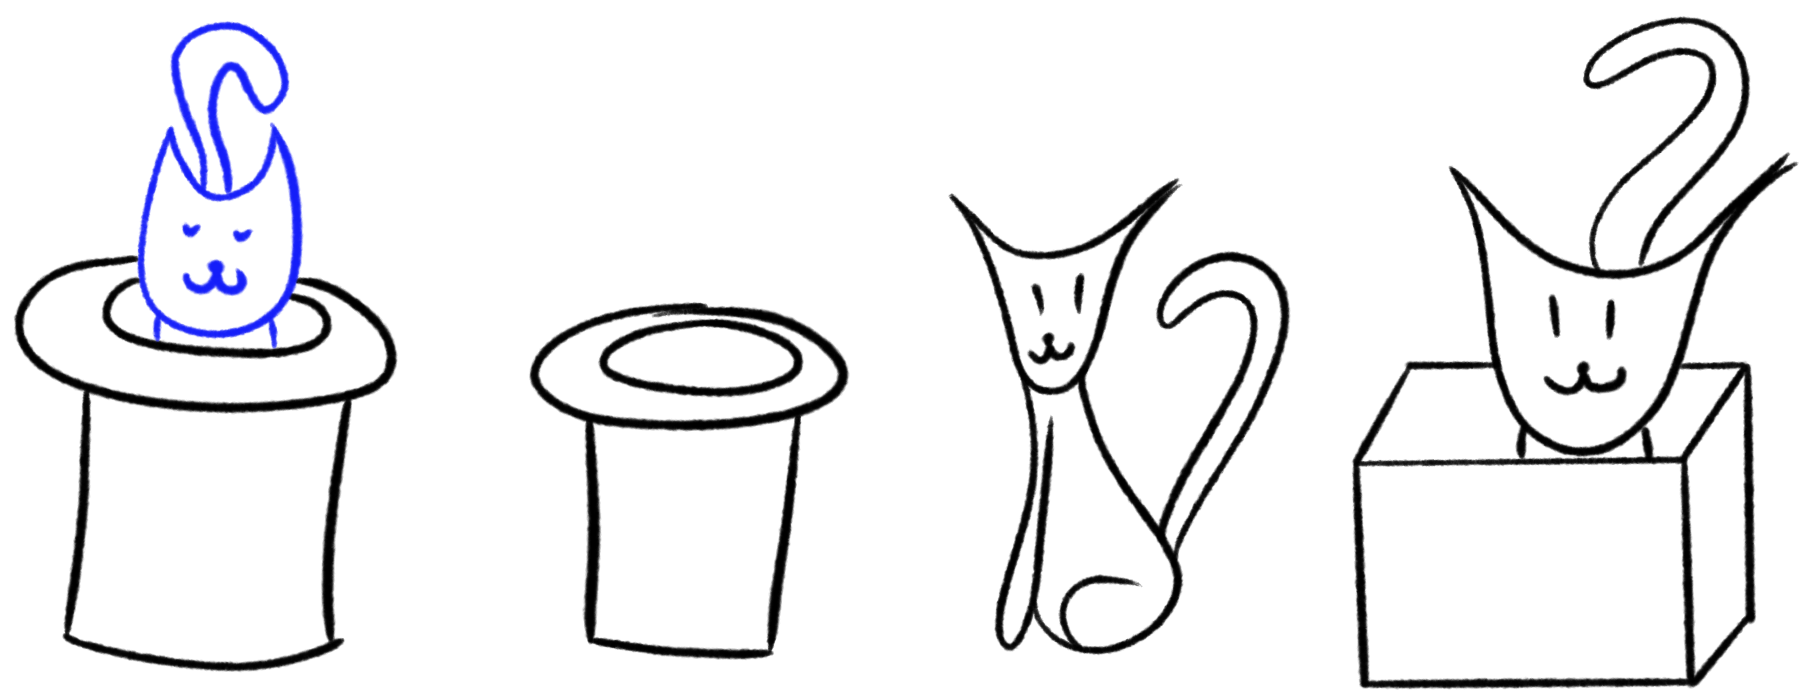
\includegraphics[width=0.95\textwidth]{figures/haddock.png}
				\caption{Haddock context, \\ several hats}\label{fig:haddock}
			\end{center}
		\end{subfigure}

		\begin{subfigure}{.5\textwidth}
			\begin{center}
				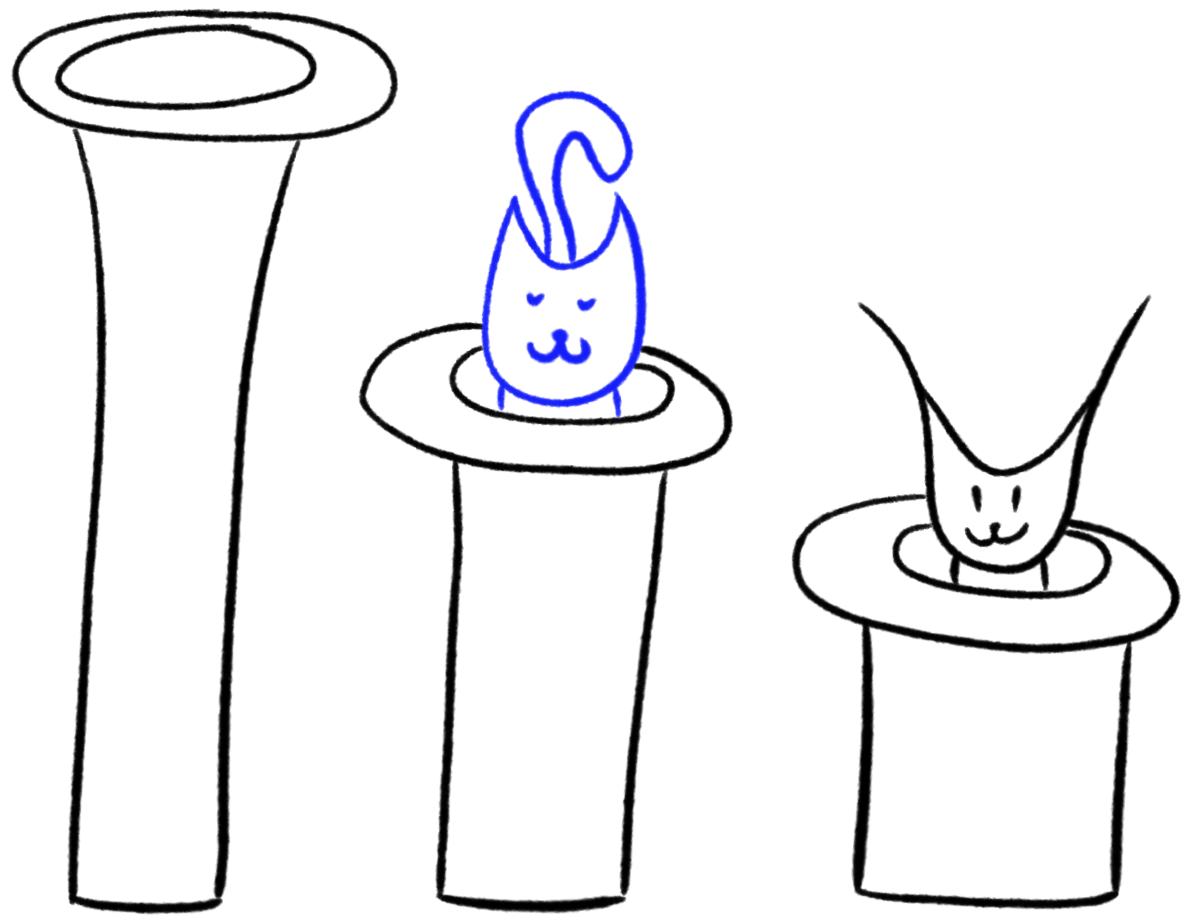
\includegraphics[width=0.76\textwidth]{figures/superlative-haddock.png}
			\end{center}
			\caption{Superlative Haddock context}\label{fig:superlative-haddock}
		\end{subfigure}%
		%
		\begin{subfigure}{.35\textwidth}
			\begin{center}
				
\includegraphics[width=.6786\textwidth]{figures/window-jumping.png}
			\end{center}
			\caption{Window jumping}
		\end{subfigure}
	\end{minipage}
	\caption{Contexts}
\end{figure}

Finally, I have novel data concerning superlative Haddock readings with regards to TRCs: First, consider a classic Haddock context of multiple hats and multiple cats, but only one hat with any cats and only one cat in any hats as in Figure~\ref{fig:haddock}; if indeed that one hatted-cat jumped out the window, (\ref{ex:haddock}) shows that TRCs may felicitously take Haddock readings.\footnote{\ok marks indicate available readings, * marks indicate unavailable readings.}

\begin{exe}
	\ex {\textbf{Haddock TRC:} \\
		The cat that there is in the hat jumps out the window.
		\begin{xlist}
			\ex {(\ok Absolute; Fig.~\ref{fig:absolute}) There is a cat in the (unique) hat. The cat jumps out the window.}
			\ex {(\ok Haddock; Fig.~\ref{fig:haddock}) There is a cat in a hat. The cat jumps out the window.\footnote{Note that a cat in the second hat would make this reading infelicitous as such would fail to satisfy uniqueness for the head determiner (i.e. item 1 in ex. \ref{ex:haddock}). This is predicted by the definite determiner at the start of the second sentence in the paraphrase (\ref{ex:haddock-sem})}}\label{ex:haddock-sem}
		\end{xlist}}\label{ex:haddock}
\end{exe}

Now, we expand our context with hats of various tall-ness and permit many cats across the hats, so long as there is only one tallest of the hats bearing any cats, and one cat in said hat as in Figure~\ref{fig:superlative-haddock} (and indeed that that cat jumped out the window), then we see (\ref{ex:sup-haddock}) may take a (relative) superlative Haddock reading.

\begin{exe}
	\ex {\textbf{(Relative) Superlative Haddock:} \\
		The cat that is in the tallest hat jumps out the window.
		\begin{xlist}
			\ex {(\ok Absolute) There is a cat in the (absolutely) tallest hat. The cat jumps out the window.\footnote{Note that Fig.~\ref{fig:superlative-haddock} is infelicitous with an absolute reading like (\ref{ex:abs-sup-sem}) since the context does not, in fact, have a cat in the absolutely tallest hat.}}\label{ex:abs-sup-sem}
			\ex {(\ok Haddock; Fig.~\ref{fig:superlative-haddock}) There is a cat in the (relatively) tallest hat with any cats in it. The cat jumps out the window.}
		\end{xlist}}\label{ex:sup-haddock}
\end{exe}

However, we see that the analogous TRC (\ref{ex:trc-sup-haddock}) is infelicitous, permitting only an absolute reading in which there is a universally tallest hat.

\begin{exe}
	\ex {\textbf{TRCed Superlative Haddock:} \\
		The cat that there is in the tallest hat jumps out the window.\\
		(\ok Absolute, * Haddock)}\label{ex:trc-sup-haddock}
\end{exe}

\subsection{Interim Summary}
To recapitulate the data just above: definites and universals determiners, but not indefinites, may generally co-occur with TRCs (\ref{ex:det}). Separately, TRCs may take plain Haddock readings (\ref{ex:haddock}) but generally not superlative Haddocks (\ref{ex:sup-haddock}).

\subsection{Hypothesis}
The present hypothesis proposes that both these effects---those determiner restrictions and superlative Haddocks---may be resolved by appealing to dynamic semantics. The head determiner selection is seen as just those determiners which regularly permit dynamic reference.

Meanwhile, the determiner associated with the superlative---`the (tallest hat)'---is split into a definite uniqueness check \(\mathbb{1}\) and indefinite introduction \(\bbexists\) following \citet{bumfordSplitscopeEffectsDefinite2017}. In this way, Haddock readings are garnered by scoping/interleaving the definiteness of hats \(\mathbb{1}_h\) over the indefiniteness of cats \(\bbexists_c\): \(\mathbb{1}_c > \mathbb{1}_h > \bbexists_h > \bbexists_h\); absolute readings flip the central relation: \(\mathbb{1}_c > \bbexists_c > \mathbb{1}_h > \bbexists_h\).
Importantly, the scope of \(\mathbb{1}\) may be trapped within the TRC, presumably by \textit{there}, such as when including superlative force. The desired results of the data should be achievable then by further considering a dynamic semantics.

\section{Planning}

My highly tentative month-by-month plan for this project is as follows:
\begin{itemize}
	\item {November: First stab at writing an analysis based on what I have researched thus far and oncoming research}
	\item {December: Continue research with focus on dynamic semantics and split scope}
	\item {January: Formalizing analysis}
	\item {February: Writing}
	\item {Mid April: First (second?) draft for feedback}
	\item {Early May: Revisions from feedback}
	\item {Late May: Ready for submission}
\end{itemize}

\printbibliography
\end{document}
